\chapter{DESARROLLO}

\section{Diseño Conceptual de la Arquitectura IIoT}
\label{sec:diseno_conceptual}

    \par El diseño conceptual del Módulo de Transmisión IoT (MT-IoT) se fundamenta en la necesidad de transformar equipos de control fiscal, tradicionalmente aislados, en nodos inteligentes capaces de integrarse a una red de monitoreo centralizada. Tal como se estableció en el plan de trabajo durante las semanas 3 y 4, el objetivo fue definir los planos técnicos y lógicos para posicionar al microcontrolador ESP32 como un puente (\textit{Gateway}) entre el hardware fiscal y la nube \cite{WEF_IIoT_2018, Connected_Everything_2016}.\\

    \par El desarrollo del proyecto se organizó en cuatro fases metodológicas sucesivas, cuyo flujo general se resume en la Figura \ref{fig:flujo_metodologico}:

    \begin{figure}[htbp]
    \centering
    \begin{tikzpicture}[node distance=0.6cm, auto, >=latex',
        phase/.style={rectangle, draw, rounded corners, fill=blue!10, text width=9.5cm, align=center, minimum height=1.0cm, font=\small},
        ar/.style={thick,->,>=stealth}]
        \node [phase] (f1) {\textbf{Fase 1.} Levantamiento de Requerimientos y Simulación HIL};
        \node [phase, below=of f1] (f2) {\textbf{Fase 2.} Detección de Inestabilidades y Cuellos de Botella (IRAM / EMI)};
        \node [phase, below=of f2] (f3) {\textbf{Fase 3.} Re-ingeniería del Kernel Concurrente (FreeRTOS / Mutex)};
        \node [phase, below=of f3] (f4) {\textbf{Fase 4.} Despliegue del Ecosistema Cloud (Django / HTMX / MQTT v5.0)};
        \draw [ar] (f1) -- (f2);
        \draw [ar] (f2) -- (f3);
        \draw [ar] (f3) -- (f4);
    \end{tikzpicture}
    \caption{Flujo metodológico general del trabajo de pasantía organizado en cuatro fases sucesivas.}
    \label{fig:flujo_metodologico}
    \end{figure}

    Para garantizar la escalabilidad y robustez del sistema (véase la Figura \ref{fig:arquitectura_iiot}), se optó por una arquitectura distribuida de tres niveles, alineada con los estándares industriales del Internet de las Cosas (IIoT) \cite{WEF_IIoT_2018, Connected_Everything_2016}:
    
    \begin{itemize}
        \item \textbf{Nivel de Borde (Edge):} Representado por la impresora fiscal HKA80. En esta capa se origina la información crítica mediante registros de estado (\texttt{Status S1}) y diagnóstico (\texttt{SV2}) \cite{TheFactoryHKA_Manual_Protocolos}. La captura de estos datos se realiza a través de una interfaz de comunicación síncrona de alto rendimiento, diseñada para operar de forma transparente. Esta transparencia se logra manteniendo un intervalo de sondeo (\textit{polling}) estrictamente acotado, asegurando que los tiempos de respuesta de la transacción no excedan los umbrales de latencia tolerados por el \textit{firmware} legal del equipo; premisa que será demostrada posteriormente mediante un perfilado de tiempos en el bus de datos.

        \item \textbf{Nivel de Pasarela (Gateway):} Ejecutado por el Módulo de Transmisión IoT (basado en el SoC ESP32). Su función es doble: actúa como maestro en la interfaz local con el periférico y como cliente seguro (\textit{Publisher}) hacia la red Wi-Fi \cite{Espressif_ESP32_Datasheet}. En este nivel se implementa la lógica de empaquetado de datos en formato JSON y la gestión de seguridad mediante TLS/SSL, permitiendo el acceso a registros críticos almacenados en la Memoria de Trabajo y Memoria de Auditoría sin interferir con el cabezal de impresión.

        \item \textbf{Nivel de Gestión y Visualización (Cloud):} Compuesto por el \textit{Broker} HiveMQ y el servidor de aplicaciones desarrollado en Django \cite{Django_v5_Doc}. Este nivel orquesta la recepción asíncrona de telemetría y su visualización en tiempo real en el Dashboard mediante un túnel de \textit{MQTT sobre WebSockets} \cite{OASIS_MQTT_v5, RFC6455_WebSockets}.
    \end{itemize}

    \begin{figure}[htbp]
        \centering
        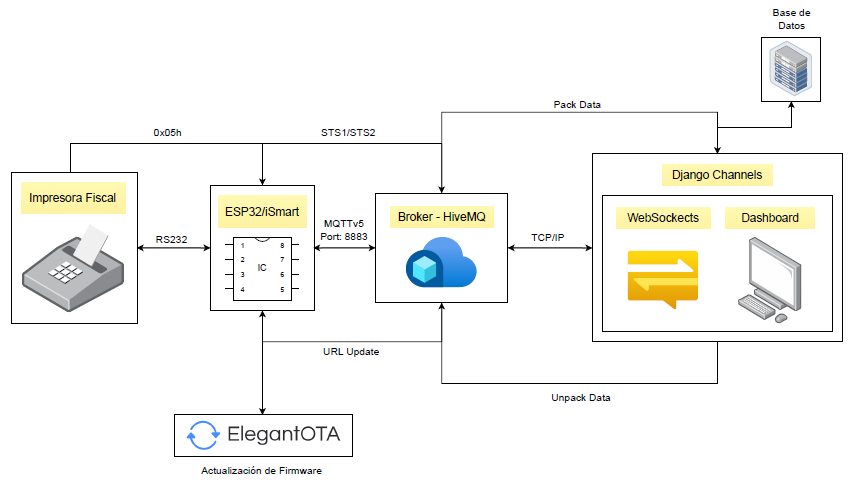
\includegraphics[width=0.95\textwidth]{Img/arquitectura_iiot.png} 
        \caption{Diagrama de la Arquitectura IIoT distribuida en tres niveles (Edge, Gateway y Cloud).}
        \label{fig:arquitectura_iiot}
    \end{figure}

    \par La elaboración de los diagramas técnicos (Figura \ref{fig:arquitectura_iiot} y Figura \ref{fig:arquitectura_mqtt}) respondió a la necesidad de visualizar el flujo de datos desde el comando inicial \texttt{0x05h} (ENQ) enviado por el MT-IoT hasta el desempaquetado (\textit{Unpack Data}) en la plataforma web \cite{Connected_Everything_2016}. El diseño de la arquitectura de comunicaciones fue especialmente crítico para definir el \textit{Topic Tree} (jerarquía de tópicos) y el uso de \textit{User Properties} de MQTT v5.0 \cite{OASIS_MQTT_v5}. La inyección de metadatos (como la versión del firmware y la intensidad de señal Wi-Fi) directamente en las \textit{User Properties} de la cabecera del protocolo evita sobrecargar el cuerpo del mensaje JSON, lo cual reduce significativamente el consumo de ancho de banda y elimina la necesidad de \textit{parsing} adicional en el servidor \cite{OASIS_MQTT_v5}.

    \begin{figure}[H]
        \centering
        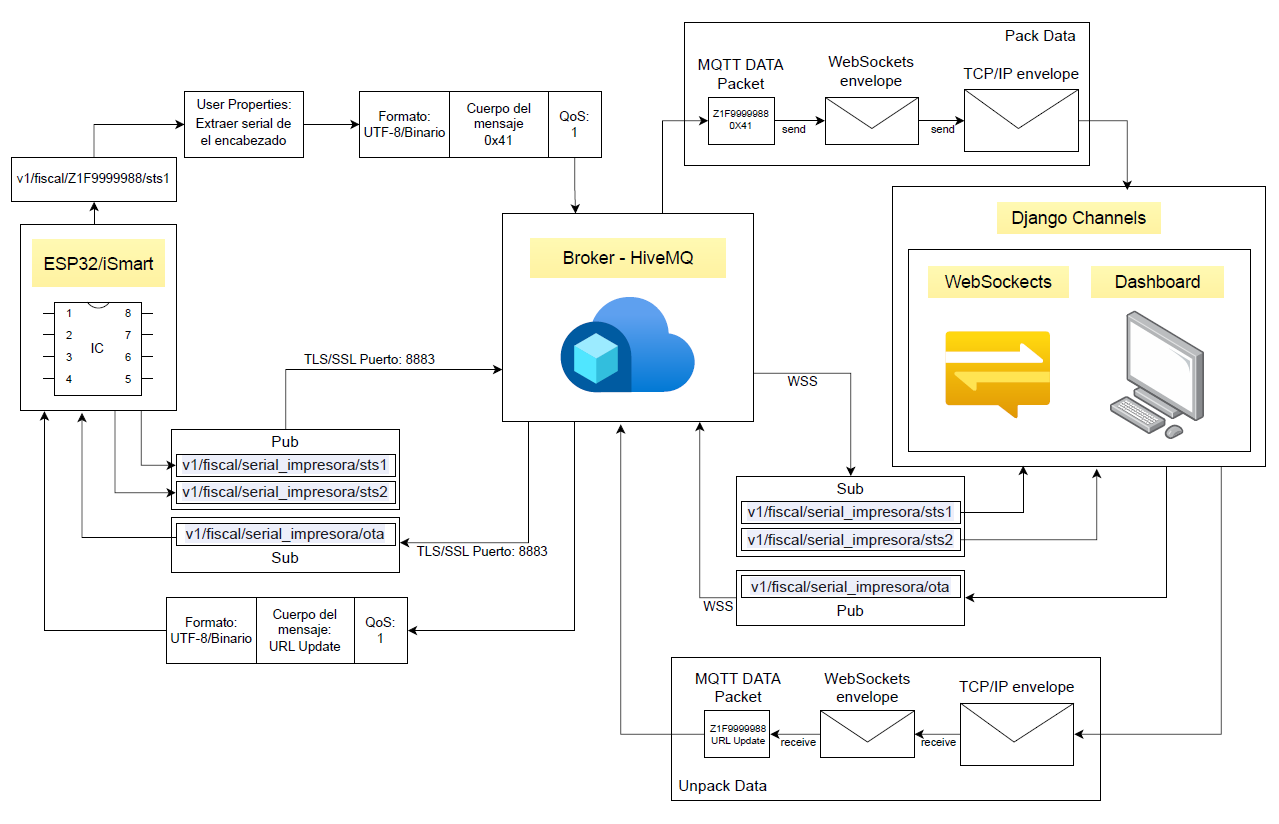
\includegraphics[width=0.95\textwidth]{Img/arquitectura_mqtt.png}
        \caption{Diagrama propuesto para la arquitectura de comunicaciones MQTT.}
        \label{fig:arquitectura_mqtt}
    \end{figure}

\section{Análisis de Decisiones de Arquitectura y Compromisos de Ingeniería}

\subsection{Microcontrolador de Doble Núcleo: ESP32}

\par Para la implementación del nodo de transmisión, se seleccionó la tarjeta de desarrollo ESP32 DevKitC V4. Esta elección se fundamentó en la necesidad de gestionar procesos concurrentes industriales \cite{Espressif_ESP32_Datasheet, FreeRTOS_Kernel_Ref}. En la arquitectura final, se asignaron tareas específicas a cada núcleo para garantizar el determinismo: mientras un núcleo gestiona el sondeo (\textit{polling}) de la impresora fiscal cada 5 segundos, el segundo núcleo administra la pila de red y la mensajería MQTT v5.0, evitando que las latencias de internet bloqueen la captura de datos locales.\\

\par Durante el prototipado, se identificó una limitación crítica en el hardware relacionada con la asignación de periféricos. Al intentar utilizar el UART1 en sus pines por defecto (GPIO 9 y 10), el sistema experimentaba reinicios constantes (bootloops) debido a que estos pines están anclados al bus SPI de la memoria Flash interna del SoC \cite{Espressif_ESP32_Datasheet}. Para solventar esta colisión eléctrica, se reconfiguró la matriz de señales, moviendo la interfaz de comunicación fiscal hacia los pines libres GPIO 18 (TX) y GPIO 19 (RX), logrando una transmisión estable (véase la Figura \ref{fig:pinlayout}).\\

\begin{figure}[htbp]
    \centering
    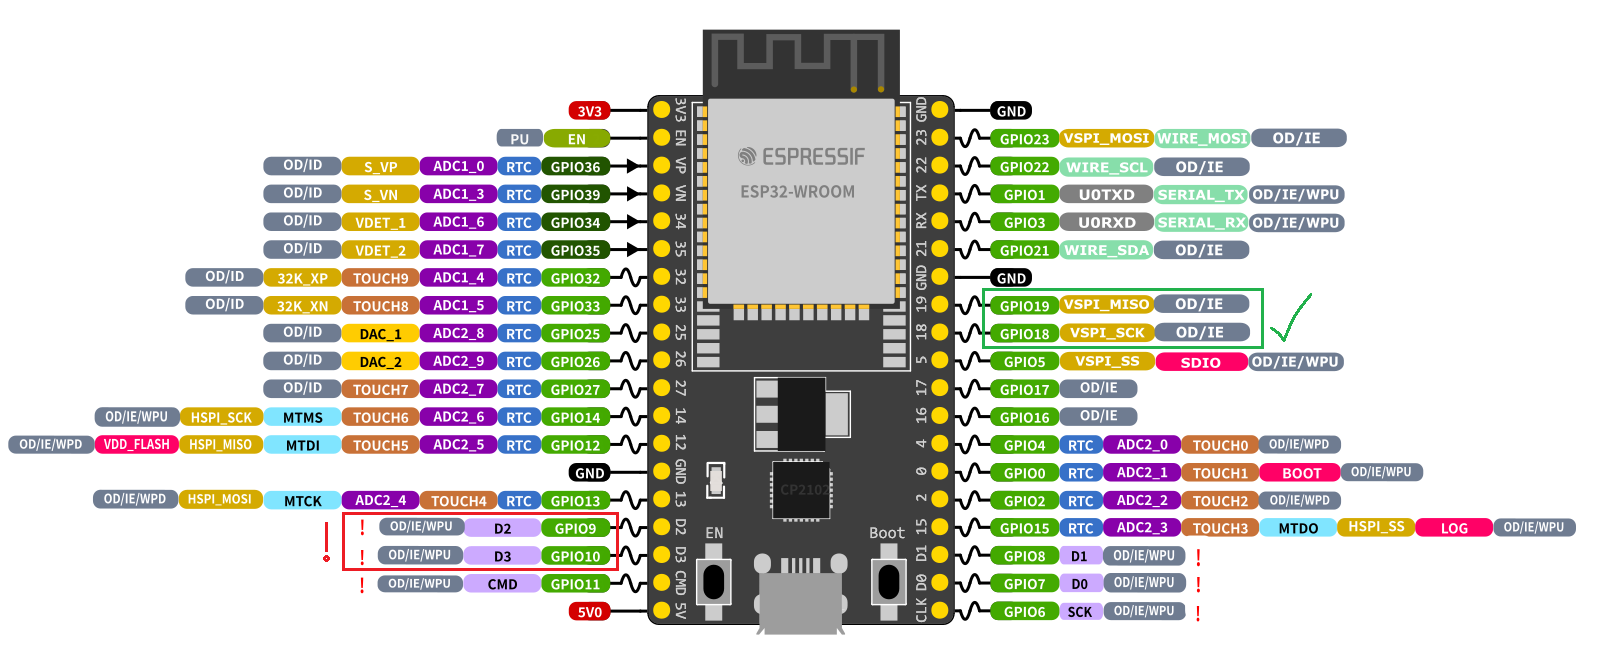
\includegraphics[width=0.8\linewidth]{Img/esp32_pinlayout.png}
    \caption{Pinlayout de la tarjeta ESP32 DevKitC V4 y reasignación de pines seriales.}
    \label{fig:pinlayout}
\end{figure}

\par La gestión de la memoria interna representó el mayor desafío técnico. Con la implementación completa de la pila TLS/SSL y el empaquetado dinámico de mensajes JSON, el uso de la memoria IRAM alcanzó un nivel crítico del 78.39\% en la semana 6. Tras un análisis de perfilado del \textit{firmware}, se aplicó una reingeniería de recursos mediante la herramienta \texttt{menuconfig} desactivando la aceleración IRAM para el \textit{stack} Wi-Fi (véase la Figura \ref{fig:menuconfig_wifi}). Esta decisión redujo el consumo de memoria a un 52.26\% (un ahorro directo del 26.13\%), liberando el \textit{heap} necesario para alojar el búfer de actualización remota (OTA).

\begin{figure}[htbp]
    \centering
    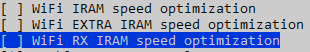
\includegraphics[width=0.5\linewidth]{Img/menuconfig_optimizacion_wifi.png}
    \caption{Configuración aplicada en menuconfig para optimización de IRAM.}
    \label{fig:menuconfig_wifi}
\end{figure}

\par Finalmente, para optimizar el consumo energético y la disipación térmica en operación continua, se aplicó una técnica de \textit{underclocking}, ajustando la frecuencia del CPU a 80 MHz (vease Figura \ref{fig:menuconfig_under}) \cite{Espressif_Menuconfig}. Esta frecuencia demostró ser estadísticamente suficiente para sostener la aceleración criptográfica de AES por hardware requerida por la conexión segura hacia HiveMQ.

\begin{figure}[htbp]
    \centering
    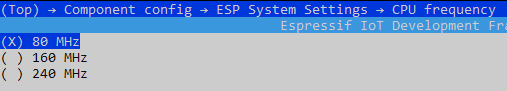
\includegraphics[width=0.7\linewidth]{Img/menuconfig_optimizacion_under.png}
    \caption{Underclocking aplicado en menuconfig para optimización de consumo energético.}
    \label{fig:menuconfig_under}
\end{figure}

\subsection{Unidad de Control Fiscal: Impresora HKA80}

\par La impresora fiscal HKA80 (véase la Figura \ref{fig:hka80}) actúa como el activo de borde (\textit{Edge}) central del sistema. Su selección se fundamentó en su arquitectura modular, la cual permite el acceso a registros críticos almacenados en su Memoria de Trabajo y Memoria de Auditoría sin interrumpir mecánicamente al cabezal de impresión.

\begin{figure}[htbp]
    \centering
    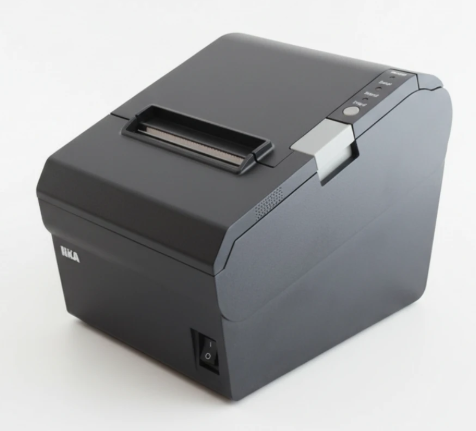
\includegraphics[width=0.6\linewidth]{Img/hka80.png}
    \caption{Impresora fiscal modelo HKA80 autorizada por la normativa vigente.}
    \label{fig:hka80}
\end{figure}

\par Para la integración con el MT-IoT, se definieron los parámetros obligatorios del protocolo: tasa de transferencia de 9600 bps, longitud de 8 bits, paridad par y 1 bit de parada \cite{TheFactoryHKA_Manual_Protocolos}. La fase inicial de la telemetría priorizó el registro \texttt{Status S1} (identidad del equipo y acumuladores) y el comando \texttt{SV2} (versión de \textit{firmware} del periférico).\\

\par Un hallazgo crítico durante el desarrollo del \textit{parser} fue la identificación de un carácter invisible de salto de línea (\texttt{\textbackslash n}) inmediatamente antes del fin de trama (ETX) emitido por la impresora. Este factor desplazaba los punteros de memoria provocando errores de tipo \textit{Off-By-One}, los cuales corrompían el \textit{payload} MQTT. La anomalía fue resuelta introduciendo un ajuste dinámico que inyecta un terminador nulo en la memoria RAM para purgar la trama. La secuencia analítica de esta corrección se describe en el Algoritmo \ref{alg:offbyone}, mientras que su implementación en lenguaje C se conserva en el Apéndice \ref{apx:codigo}.

\begin{algorithm}[htbp]
\caption{Mitigación analítica del error Off-By-One en el parseo de la trama SV2.}
\label{alg:offbyone}
\begin{algorithmic}[1]
\State Recibir el bloque de respuesta y validar su redundancia (LRC).
\State Calcular la posición del terminador: $p_{ETX} \leftarrow n - 2$.
\State Estimar el índice inicial del campo de versión: $i_0 \leftarrow p_{ETX} - L_{fw} - 1$.
\If{$i_0 \geq 1$}
    \State Reservar la sección crítica de memoria.
    \State Copiar $L_{fw}$ caracteres desde $i_0$ hacia el campo de versión.
    \State Inyectar el terminador nulo manual en la posición $L_{fw}$.
    \State Liberar la sección crítica.
    \State \Return verdadero
\EndIf
\State \Return falso
\end{algorithmic}
\end{algorithm}

\par Esta sanitización de datos asegura un determinismo absoluto en la captura de registros cada 5 segundos, permitiendo que el MT-IoT actúe como un \textit{Gateway} transparente que no añade latencia a la red transaccional del contribuyente.

\subsection{Justificación del Framework Nativo: Determinismo vs. Latencia (ESP-IDF)}

\par Durante la semana de definición tecnológica se realizó un análisis comparativo entre el entorno Arduino IDE y el Espressif IoT Development Framework (ESP-IDF) (véase la Tabla \ref{tab:comparativa_frameworks}).\\

\begin{table}[htbp]
    \centering
    \caption{Análisis comparativo de entornos de desarrollo para el nodo Gateway.}
    \label{tab:comparativa_frameworks}
    \begin{tabularx}{\textwidth}{@{}>{\raggedright\arraybackslash}p{3.0cm} >{\raggedright\arraybackslash}X >{\raggedright\arraybackslash}X@{}}
        \toprule
        \textbf{Criterio} & \textbf{Arduino IDE} & \textbf{ESP-IDF v5.5.2} \\
        \midrule
        Modelo de Ejecución & Bucle secuencial único (\texttt{setup/loop}). & Multitarea concurrente (\texttt{app\_main}). \\
        Gestión de Tareas & Dependiente de bloqueos (\texttt{delay}). & Planificación RTOS (\texttt{xTaskCreate}). \\
        Gestión de Memoria & Compilación estandarizada, alta redundancia. & Control sobre componentes vía \texttt{menuconfig}. \\
        Idoneidad & Prototipado rápido, baja escalabilidad. & Despliegue industrial y seguridad TLS. \\
        \bottomrule
    \end{tabularx}
\end{table}

\par La elección del framework de desarrollo representó un compromiso (\textit{trade-off}) crítico entre velocidad de prototipado y determinismo temporal. Aunque el ecosistema Arduino permitía un despliegue ágil, su modelo de ejecución mono-hilo imponía latencias inaccesibles. En un entorno transaccional fiscal, un retardo provocado por un \texttt{delay()} bloqueante en el stack Wi-Fi arriesgaba sobrepasar la ventana temporal de lectura del firmware fiscal legal. Por ello, se justificó el uso nativo de \textbf{ESP-IDF}, permitiendo gestión explícita de memoria en C y la asignación determinista de tareas mediante FreeRTOS.\\

\par Si bien Arduino ofrece una curva de aprendizaje reducida, su modelo de ejecución secuencial representa un cuello de botella sistémico. Al optar por ESP-IDF \cite{Espressif_ESP_IDF_v552}, la migración del punto de entrada del programa hacia \texttt{app\_main} permitió el despliegue de la API de FreeRTOS. A través de la función \texttt{xTaskCreatePinnedToCore} \cite{FreeRTOS_Kernel_Ref}, se logró orquestar tareas independientes fijadas a núcleos específicos, garantizando que el \textit{stack} de red no interrumpiera la captura local por UART.\\

\par Adicionalmente, el sistema de construcción CMake permitió una declaración explícita de componentes (editando el archivo \texttt{CMakeLists.txt}, véase la Figura \ref{fig:dirs}), asegurando que solo se incluyeran dependencias estrictamente necesarias como \texttt{esp\_https\_ota} y \texttt{mqtt}. Estas decisiones de ingeniería permitieron que el ESP32 operara con una arquitectura modular y determinista.

\begin{figure}[htbp]
    \centering
    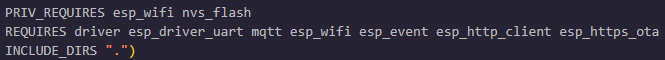
\includegraphics[width=0.9\linewidth]{Img/cmakelist_dirs.png}
    \caption{Inclusión estricta de dependencias en el archivo de construcción CMakeLists.txt.}
    \label{fig:dirs}
\end{figure}

\section{Fase de Prototipado y Simulación Inicial}

\par El desarrollo de la primera fase del sistema de transmisión comenzó con un enfoque de validación incremental, motivado principalmente por la indisponibilidad inicial de la interfaz de desarrollo física de la impresora fiscal corporativa \cite{TheFactoryHKA_iSmart_Manual}. Para mitigar este cuello de botella y asegurar el progreso del cronograma técnico, se diseñó una metodología de simulación por software que permitió emular el comportamiento del hardware de borde (\textit{Edge}) y verificar los cimientos del \textit{firmware} en un entorno controlado antes de la integración física final \cite{TheFactoryHKA_iSmart_Manual}.

\subsection{Configuración de la Comunicación Asíncrona (UART)}

\par La comunicación física inicial entre el MT-IoT y la unidad fiscal se estructuró bajo el estándar asíncrono RS-232, utilizando los parámetros serie nativos del hardware \cite{TheFactoryHKA_Manual_Protocolos}. Al no contar con el periférico real en el laboratorio, se empleó un computador personal como activo de simulación, lo que requirió la estructuración de dos entornos de prueba sucesivos:

\begin{enumerate}
    \item \textbf{Pruebas con Terminales de Datos (RealTerm):} En primera instancia, se intentó inyectar y monitorear tramas de datos binarios de forma manual. Si bien este método permitió verificar respuestas básicas al comando \textit{Enquiry} (\texttt{ENQ = 0x05h}), tal como se aprecia en la Figura \ref{fig:enq_realterm}, la herramienta resultó inviable por conflictos de codificación: la consola presentaba limitaciones para concatenar de forma determinista caracteres hexadecimales puros (como los terminadores \texttt{STX 0x02} y \texttt{ETX 0x03}) con los 129 bytes de texto ASCII requeridos para emular una respuesta válida del \texttt{Status S1} \cite{TheFactoryHKA_Manual_Protocolos}.
    
    
    \item \textbf{Simulador Dedicado en Python:} Para solventar el problema de codificación mixta, se programó un \textit{script} de automatización nativo utilizando la biblioteca \texttt{pyserial}. Este programa simuló de manera fidedigna los registros de la impresora (a 9600 bps, 8 bits, paridad par y 1 bit de parada), interceptando solicitudes seriales y estructurando dinámicamente respuestas válidas, tal como se evidencia en la máquina de estados de la Figura \ref{fig:fsm_simulador} (el listado del programa se conserva en el Apéndice \ref{apx:codigo}).
\end{enumerate}

\begin{figure}[htbp]
    \centering
    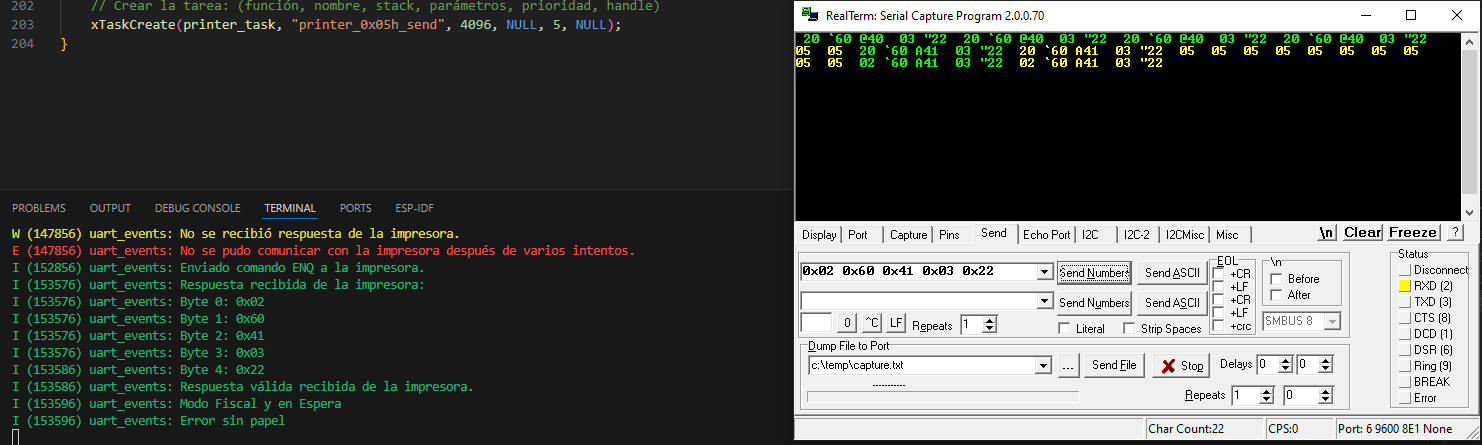
\includegraphics[width=0.95\textwidth]{Img/enq_realterm.png}
    \caption{Captura de inyección manual de tramas y comando ENQ mediante la terminal de datos RealTerm.}
    \label{fig:enq_realterm}
\end{figure}

\begin{figure}[htb]
\centering
\resizebox{0.8\textwidth}{!}{%
\begin{tikzpicture}[node distance=1.7cm, auto, >=latex',
    proc/.style={rectangle, draw, rounded corners, fill=blue!10, text width=3.4cm, align=center, minimum height=1.0cm, font=\small},
    dec/.style={diamond, draw, fill=orange!15, aspect=2.6, align=center, inner sep=1pt, font=\small},
    ar/.style={thick,->,>=stealth}]
    \node [proc] (rx) {Recepción del bloque (STX \ldots ETX)};
    \node [proc, below=of rx] (lrc) {Cálculo del LRC acumulado (XOR)};
    \node [dec, below=of lrc] (dec) {¿LRC válido?};
    \node [proc, below left=1.3cm and 1.4cm of dec] (ack) {Respuesta ACK (0x06)};
    \node [proc, below right=1.3cm and 1.4cm of dec] (nak) {Respuesta NAK (0x15)};
    \draw [ar] (rx) -- (lrc);
    \draw [ar] (lrc) -- (dec);
    \draw [ar] (dec) -- node[left, font=\scriptsize]{sí} (ack);
    \draw [ar] (dec) -- node[right, font=\scriptsize]{no} (nak);
\end{tikzpicture}%
}
\caption{Máquina de estados del simulador fiscal en software.}
\label{fig:fsm_simulador}
\end{figure}

\vspace{0.5cm}

\par En el entorno del MT-IoT, bajo el núcleo del RTOS, se implementó la tarea base denominada \texttt{printer\_polling\_task} \cite{FreeRTOS_Kernel_Ref}. El aspecto clave de esta rutina fue la sustitución de los retardos secuenciales bloqueantes por una cesión voluntaria del control al planificador (véase el Algoritmo \ref{alg:polling}) \cite{FreeRTOS_Kernel_Ref}. Al utilizar la macro \texttt{pdMS\_TO\_TICKS}, el planificador suspende la tarea durante la ventana de $5000\text{ ms}$, liberando tiempo de CPU para que el segundo núcleo procese el \textit{stack} de red sin interrupciones \cite{FreeRTOS_Kernel_Ref}.

\begin{algorithm}[htbp]
\caption{Tarea de interrogación serial no bloqueante.}
\label{alg:polling}
\begin{algorithmic}[1]
\State Inicializar la tarea de sondeo fiscal.
\While{verdadero}
    \State Transmitir el carácter de encuesta \texttt{ENQ} (0x05) por el bus local.
    \State Ceder el control al planificador durante $T_{s} = 5000$~ms.
\EndWhile
\end{algorithmic}
\end{algorithm}

\subsection{Integración de Mensajería Ligera (MQTT sobre TCP)}

\par Una vez consolidada la captura de datos locales, el desarrollo se orientó a la capa de transporte. Previo a la implementación final, se realizó una validación enviando tramas crudas mediante peticiones \texttt{HTTP GET} hacia la nube, lo que confirmó el correcto dimensionamiento del \textit{heap} para el \textit{stack} de red Wi-Fi de ESP-IDF \cite{Espressif_ESP_IDF_v552}.\\

\par Sin embargo, para cumplir con los requerimientos industriales de mínima sobrecarga (\textit{overhead}) de cabecera y envío asíncrono, se migró hacia el estándar MQTT v5.0 sobre conexiones TCP/IP \cite{OASIS_MQTT_v5}. El prototipado inicial utilizó el \textit{broker} de código abierto \textit{Eclipse Mosquitto} en el entorno local (puerto estándar 1883 no cifrado) \cite{OASIS_MQTT_v5}.\\

\par El \textit{firmware} orquestó la conexión mediante el bucle de eventos \texttt{mqtt\_event\_handler}. Al recibir la confirmación de conexión (\texttt{MQTT\_EVENT\_CONNECTED}), el sistema disparaba la tarea de publicación a través del nivel de calidad de servicio \texttt{QoS 1} (entrega garantizada al menos una vez). Las pruebas operativas se realizaron empaquetando el \texttt{Status S1} simulado en cadenas JSON planas hacia una jerarquía preliminar de tópicos, sentando las bases para el modelado asíncrono y los mecanismos de persistencia del servidor web final \cite{Django_v5_Doc}.\\

\par La efectividad de este canal de transporte se validó mediante la intercepción del \textit{payload} en el \textit{Broker} HiveMQ. Tal como se documenta en la Tabla \ref{tab:json_s1}, el microcontrolador logró empaquetar exitosamente los registros crudos de la impresora en una estructura clave-valor legible, confirmando la correcta extracción del RIF, los acumuladores de ventas y los estados operativos. El listado textual del mensaje se conserva en el Apéndice \ref{apx:codigo}.

\begin{table}[htbp]
\centering
\caption{Estructura del mensaje JSON del \texttt{Status S1} publicado hacia el \textit{broker} MQTT.}
\label{tab:json_s1}
\begin{tabularx}{\textwidth}{@{}l l >{\raggedright\arraybackslash}X@{}}
\toprule
\textbf{Clave} & \textbf{Tipo} & \textbf{Descripción} \\
\midrule
\texttt{timestamp} & Entero & Marca temporal del RTOS en milisegundos \\
\texttt{sts1} & Cadena & Estado lógico del equipo (p. ej., \texttt{0x60}) \\
\texttt{sts2} & Cadena & Estado del mecanismo de impresión (p. ej., \texttt{0x40}) \\
\texttt{estado} & Cadena & Descripción textual del estado lógico \\
\texttt{error} & Cadena & Descripción textual del error mecánico \\
\texttt{cajero} & Cadena & Identificador del cajero (ATM) \\
\texttt{ventas} & Cadena & Acumulador de ventas diarias \\
\texttt{fact\_emitidas} & Cadena & Contador de facturas emitidas \\
\texttt{rif} & Cadena & Registro de Información Fiscal del contribuyente \\
\texttt{registro} & Cadena & Número de registro de la máquina \\
\bottomrule
\end{tabularx}
\end{table}

\section{Diagnóstico e Identificación de Inestabilidades en Entornos Industriales Hostiles}

\par A medida que el \textit{firmware} del Módulo de Transmisión IoT (MT-IoT) incorporó las capas de seguridad criptográfica y la lógica de transporte hacia la nube, el sistema comenzó a exhibir cuellos de botella operativos y fallos de estabilidad. Esta sección analiza las limitaciones críticas identificadas en el hardware y el software durante las pruebas de estrés en condiciones operativas, las cuales comprometían el determinismo y la alta disponibilidad exigidas para un dispositivo industrial \cite{Connected_Everything_2016}.

\subsection{Restricciones de Memoria y Gestión de la pila IRAM}

\par La integración de una comunicación segura basada en cifrado de clave pública hacia el \textit{Broker} requirió la habilitación de la pila de seguridad Mbed TLS nativa de ESP-IDF \cite{Espressif_ESP_IDF_v552}. Sin embargo, la inicialización del \textit{handshake} TLS/SSL, la validación de certificados raíz para HiveMQ Cloud y el procesamiento dinámico de objetos mediante la librería \texttt{cJSON} generaron un consumo exponencial de memoria en el microcontrolador \cite{FreeRTOS_Kernel_Ref}.\\

\par En la arquitectura del SoC ESP32, la memoria interna SRAM de 520 KB se divide lógicamente en segmentos de instrucción (IRAM) y de datos (DRAM) \cite{Espressif_ESP32_Datasheet}. Durante las pruebas de estrés con la pila segura y el cliente de telemetría activos, el uso de la IRAM escaló críticamente hasta alcanzar el 78.39\% (102,751 Bytes utilizados de 131,072 Bytes disponibles), dejando un estrecho margen operativo, tal como se evidencia en la Figura \ref{fig:iram_crisis}.

\begin{figure}[htbp]
    \centering
    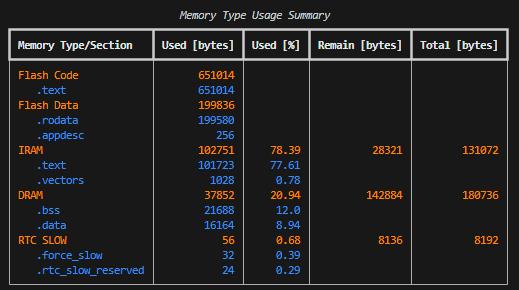
\includegraphics[width=0.75\linewidth]{Img/iram_crisis.png}
    \caption{Perfilado de memoria revelando un nivel crítico de ocupación de la IRAM (78.39\%).}
    \label{fig:iram_crisis}
\end{figure}

\par Este escenario de alta ocupación presentaba riesgos técnicos severos:

\begin{itemize}
    \item \textbf{Desbordamiento de Pila (\textit{Stack Overflow}):} El planificador de tareas de FreeRTOS quedaba vulnerable ante picos de tráfico de red o lazos de reconexión asíncronos, donde cualquier asignación de pila adicional provocaría un reinicio crítico del sistema por pánico del \textit{kernel}.
    
    \item \textbf{Inviabilidad del Sistema de Actualización (OTA):} La saturación de memoria impedía reservar el espacio dinámico (\textit{heap}) requerido para alojar los \textit{buffers} de descarga del cliente HTTP, imposibilitando la orquestación de la tabla de particiones dual (Factory + 2 OTA).
\end{itemize}

\subsection{Interferencia Electromagnética y Basura en el Bus UART}

\par En la etapa de prototipado inicial, la captura local de datos fiscales se realizaba utilizando el transceptor asíncrono UART \cite{TheFactoryHKA_Manual_Protocolos}. Al implementar el flujo bidireccional estricto gobernado por caracteres de control físicos (\texttt{ACK 0x06h} y \texttt{NAK 0x15h}), se evidenció que este estándar presentaba vulnerabilidades inaceptables para la robustez industrial.\\

\par Debido a la ausencia de blindaje electromagnético en el cable de interconexión local y la naturaleza asíncrona del bus, las líneas físicas actuaban como antenas ante el ruido y la interferencia electromagnética (EMI) del entorno. Esta inyección de ruido deformaba los bits de datos en tránsito, insertando "basura" en el controlador de hardware del microcontrolador.\\

\par Al alterarse las tramas físicas (especialmente los 129 bytes del comando \texttt{Status S1}), el \textit{firmware} fallaba en la comprobación matemática de redundancia longitudinal (LRC) \cite{TheFactoryHKA_Manual_Protocolos}. Para mitigar temporalmente este fenómeno antes de la migración definitiva a la interfaz síncrona, se implementó una estricta validación por \textit{software} que descartaba las tramas corruptas y liberaba el bus, tal como se documenta en el Algoritmo \ref{alg:lrc}.

\begin{algorithm}[htbp]
\caption{Validación de integridad de trama e intercepción de ruido electromagnético.}
\label{alg:lrc}
\begin{algorithmic}[1]
\State Recibir la trama $(STX, D, ETX, LRC_{rx})$.
\If{$STX \neq \texttt{0x02}$ \textbf{o} $ETX \neq \texttt{0x03}$}
    \State Enviar \texttt{NAK} y descartar la trama.
\EndIf
\State Calcular $LRC_{calc} \leftarrow \bigoplus_{i=1}^{n-1} b_i$.
\If{$LRC_{rx} = LRC_{calc}$}
    \State Enviar \texttt{ACK}.
\Else
    \State Enviar \texttt{NAK}, incrementar el contador de errores y liberar el bus.
\EndIf
\end{algorithmic}
\end{algorithm}

\subsection{Problemas de Concurrencia (Race Conditions)}

\par La orquestación multitarea de FreeRTOS permite ejecutar procesos de forma paralela en los dos núcleos del ESP32 \cite{FreeRTOS_Kernel_Ref}. Sin embargo, la coexistencia de la tarea de adquisición fiscal continua y la recepción de comandos inalámbricos introdujo condiciones de carrera (\textit{Race Conditions}) severas:

\begin{enumerate}
    \item \textbf{Colisiones Eléctricas (\say{Choque de Trenes}):} Durante las pruebas iniciales de actualización, si el microcontrolador recibía un comando de descarga OTA por MQTT exactamente en el mismo milisegundo en que la tarea fiscal iniciaba su ciclo de sondeo, ambas rutinas intentaban polarizar las líneas físicas locales simultáneamente. Al carecer de exclusión mutua coordinada a nivel de \textit{hardware}, el controlador entraba en pánico (lanzando una excepción \texttt{assert failed}) y forzaba el reinicio de la placa (véase la Figura \ref{fig:choque_trenes}).
    
    \item \textbf{Lecturas Cruzadas (\textit{Corrupción de RAM}):} A nivel lógico, la tarea de monitoreo sobrescribía continuamente los acumuladores de ventas en los búferes de la memoria RAM. Si la tarea MQTT despertaba de manera asíncrona para empaquetar el \textit{payload} JSON en ese preciso lapso, leía una mezcla de datos viejos y nuevos, transmitiendo telemetría fiscal híbrida y corrupta hacia el servidor.
\end{enumerate}

\begin{figure}[htbp]
\centering
\begin{tikzpicture}[>=latex',
    task/.style={rectangle, draw, rounded corners, fill=blue!10, minimum width=3.6cm, minimum height=1.1cm, align=center, font=\small},
    bus/.style={rectangle, draw, fill=orange!20, minimum width=3.2cm, minimum height=1.4cm, align=center, font=\small},
    ev/.style={rectangle, draw, fill=red!15, rounded corners, minimum width=3.6cm, minimum height=1.0cm, align=center, font=\scriptsize},
    ar/.style={thick,->,>=stealth}]
    \node [task] (poll) at (0,2.2) {Tarea \texttt{Polling}\\ (sondeo fiscal $S1$)};
    \node [task] (ota) at (0,-0.2) {Tarea \texttt{OTA}\\ (reescritura de firmware)};
    \node [bus] (bus) at (6.2,1.0) {Bus SPI local\\(pines compartidos)};
    \node [ev] (crash) at (6.2,-1.9) {\texttt{assert failed}\\reinicio del SoC};
    \draw [ar, red] (poll.east) -- node[above, font=\scriptsize, text=red]{$t_0$} (bus.west);
    \draw [ar, red] (ota.east) -- node[below, font=\scriptsize, text=red]{$t_0$} (bus.west);
    \draw [ar] (bus.south) -- (crash.north);
    \node [font=\scriptsize, text=red, align=center] at (3.1,-1.9) {acceso simultáneo\\sin mutex};
\end{tikzpicture}
\caption{Traza de depuración y registro de evento ante colisión por acceso concurrente al bus local (Choque de Trenes).}
\label{fig:choque_trenes}
\end{figure}

\par Estas limitaciones demostraron empíricamente que, para un entorno de control tributario, no basta con lograr comunicación bidireccional; es mandatorio implementar mecanismos de exclusión mutua por \textit{hardware} (como \textit{Mutexes}) y optimizaciones granulares de la memoria \cite{Espressif_ESP32_Datasheet}.

\section{Diseño de un Kernel Concurrente e Invariante de Red a Prueba de Condiciones de Carrera}

\par Una vez identificados los cuellos de botella en la gestión de memoria, la vulnerabilidad al ruido eléctrico de la línea de datos asíncrona y las condiciones de carrera en los hilos de FreeRTOS, se procedió a realizar una re-ingeniería profunda sobre los cimientos del \textit{firmware} del MT-IoT \cite{Espressif_ESP_IDF_v552}. Esta fase se enfocó en reestructurar la capa de abstracción de \textit{hardware} y optimizar el planificador de tareas de tiempo real para asegurar el determinismo y la resiliencia del sistema en entornos industriales hostiles.

\subsection{Implementación de la Interfaz Síncrona de Alto Rendimiento}

\par Para mitigar la inyección de bytes corruptos generada por la susceptibilidad electromagnética del estándar asíncrono, se migró la interconexión física local hacia una interfaz de comunicación serie síncrona dedicada, operando a una frecuencia de 100 kHz \cite{Espressif_ESP32_Datasheet}. A diferencia de la comunicación UART anterior, este método basa el muestreo de datos en una señal de temporización (\textit{Clock}) dedicada, generada por el ESP32 en rol de maestro, eliminando de raíz las desviaciones por deriva de reloj (\textit{baud-rate drift}) y garantizando una transmisión determinista \cite{Espressif_ESP_IDF_v552}. La disposición física de este enlace maestro-esclavo se ilustra en la Figura \ref{fig:bus_sincrono}.\\

\begin{figure}[htbp]
\centering
\begin{tikzpicture}[>=latex',
    box/.style={rectangle, draw, rounded corners, fill=blue!10, minimum width=2.8cm, minimum height=2.6cm, align=center, font=\small},
    lbl/.style={font=\scriptsize, inner sep=1pt}]
    \node [box] (m) {ESP32\\[3pt]\textit{Maestro}};
    \node [box, right=6.5cm of m] (s) {Periférico Fiscal\\[3pt]\textit{Esclavo}};
    \draw [->] ([yshift=20pt]m.east) -- node[above, lbl]{(reloj, 100 kHz)} ([yshift=20pt]s.west);
    \draw [->] ([yshift=7pt]m.east) -- node[above, lbl]{(habilitación del esclavo)} ([yshift=7pt]s.west);
    \draw [->] ([yshift=-7pt]m.east) -- node[below, lbl]{(datos de transmisión)} ([yshift=-7pt]s.west);
    \draw [->] ([yshift=-20pt]s.west) -- node[below, lbl]{(datos de recepción)} ([yshift=-20pt]m.east);
\end{tikzpicture}
\caption{Interacción maestro-esclavo sobre el bus síncrono local, con señal de reloj dedicada a 100 kHz y vías independientes de transmisión y recepción.}
\label{fig:bus_sincrono}
\end{figure}

\par Para blindar la integridad lógica de las tramas tributarias en esta nueva capa física, se implementó una rutina matemática de validación de redundancia longitudinal (LRC). Tras recibir cada bloque de datos, el \textit{firmware} ejecuta un lazo cerrado que realiza operaciones lógicas \texttt{XOR} acumulativas sobre los bytes recibidos, contrastando el resultado con el \textit{checksum} enviado por el periférico fiscal \cite{TheFactoryHKA_Manual_Protocolos}.\\

\par Si la trama es declarada válida, el MT-IoT responde con un carácter \texttt{ACK (0x06h)}; de lo contrario, envía un \texttt{NAK (0x15h)} y procede de inmediato a reiniciar lógicamente los registros del hardware del bus local, impidiendo la propagación de datos corruptos en la memoria del sistema.\\

\par Adicionalmente, para evitar bloqueos del procesador si el periférico es apagado físicamente, se establecieron temporizadores (\textit{timeouts}) estrictos. Si se supera el límite de fallos continuos, el \textit{firmware} transiciona al estado de pánico y activa una máquina de reconexión, sin bloquear las tareas de red \cite{FreeRTOS_Kernel_Ref}.

\subsection{Orquestación Concurrente mediante FreeRTOS}

\par El control cooperativo del MT-IoT se organizó bajo el \textit{kernel} de FreeRTOS mediante un esquema de exclusión mutua de dos niveles, solventando la condición de carrera identificada en la etapa de prototipado:

\begin{enumerate}
    \item \textbf{Exclusión Mutua de Datos en RAM (\texttt{mqtt\_data\_mutex}):} Se implementó un semáforo tipo \textit{Mutex} para proteger la estructura \texttt{mqtt\_data\_t} en la DRAM. Este candado lógico garantiza que la tarea de monitoreo local no pueda sobrescribir variables de facturación mientras la tarea MQTT está leyendo el bloque para formatear el \textit{payload} JSON, evitando el tránsito de datos híbridos.
    
    \item \textbf{Exclusión Mutua del Bus Físico (\texttt{bus\_local\_mutex}):} Para resolver la colisión eléctrica local (choque de trenes) cuando una actualización remota coincide con el sondeo periódico de 5 segundos, se introdujo un segundo \textit{Mutex} de \textit{hardware}. Como se observa en la Figura \ref{fig:mutex_doble}, tanto la tarea de sondeo como la rutina OTA deben competir y adquirir con éxito este semáforo antes de poder energizar el canal de comunicación físico. El listado de la implementación se conserva en el Apéndice \ref{apx:codigo}.
\end{enumerate}

\begin{figure}[htb]
\centering
\begin{tikzpicture}[node distance=1.3cm, auto, >=latex',
    proc/.style={rectangle, draw, rounded corners, fill=blue!10, text width=6cm, align=center, minimum height=1.0cm, font=\small},
    dec/.style={diamond, draw, fill=orange!15, aspect=3.2, align=center, inner sep=1pt, font=\small},
    ar/.style={thick,->,>=stealth}]
    \node [proc] (ini) {Solicitud de acceso al bus local};
    \node [dec, below=of ini] (m1) {¿Mutex del bus?};
    \node [proc, below=of m1] (val) {Validación de la trama (LRC)};
    \node [dec, below=of val] (m2) {¿Mutex de datos?};
    \node [proc, below=of m2] (wr) {Escritura en la estructura de telemetría};
    \node [proc, below=of wr] (rel) {Liberación de ambos semáforos};
    \draw [ar] (ini) -- (m1);
    \draw [ar] (m1) -- node[right, font=\scriptsize]{sí} (val);
    \draw [ar] (val) -- (m2);
    \draw [ar] (m2) -- node[right, font=\scriptsize]{sí} (wr);
    \draw [ar] (wr) -- (rel);
\end{tikzpicture}
\caption{Exclusión mutua en dos niveles para la protección de la memoria RAM y del bus físico.}
\label{fig:mutex_doble}
\end{figure}

\par Para proteger la memoria (\textit{heap}) ante ráfagas de comandos MQTT, la lógica OTA se desacopló del bucle principal. Se creó la tarea \texttt{ota\_supervisor\_task}. Al detectarse un comando de actualización, el manejador MQTT empuja la solicitud a una cola segura (\texttt{ota\_cmd\_queue}). Al despertar, el supervisor activa una bandera global de \say{freno de mano} (\texttt{ota\_en\_progreso = true}) que paraliza la tarea fiscal, y ejecuta la descarga en total aislamiento \cite{Espressif_ESP_IDF_v552}.

\subsection{Estrategias de Resiliencia de Red y DNS Injection}

\par Para cumplir con los requerimientos de robustez industrial, el \textit{firmware} se dotó de mecanismos de autodefensa. Ante cortes del proveedor de internet (ISP), la capa de red del microcontrolador gatilla asíncronamente el evento \texttt{WIFI\_EVENT\_STA\_DISCONNECTED}, iniciando un lazo de reconexión infinito que intenta reanudar el enlace sin reiniciar la lógica de control interna \cite{Espressif_ESP_IDF_v552}.\\

\par Uno de los aportes más significativos fue la mitigación de fallos de resolución de nombres (\textit{DNS}) del contribuyente. Al capturar una dirección IP local a través del evento \texttt{IP\_EVENT\_STA\_GOT\_IP}, la pasarela intercepta dinámicamente la configuración de la interfaz de red (\textit{netif}) e inyecta forzosamente los servidores principales de Google (8.8.8.8) \cite{Espressif_ESP_IDF_v552}. Esta técnica asegura que el cliente TLS siempre resuelva la ruta hacia HiveMQ.\\

\par Finalmente, ante caídas temporales del servidor MQTT, el \textit{firmware} impone un retardo de cortesía (\texttt{RECONNECT\_DELAY\_MS}) antes de intentar levantar el \textit{socket} nuevamente (véase el Algoritmo \ref{alg:reconexion}). Esto evita ataques de denegación de servicio (DDoS) involuntarios contra el \textit{Broker} y estabiliza el consumo energético del MT-IoT.

\begin{algorithm}[htbp]
\caption{Resiliencia y reconexión no bloqueante en la tarea MQTT.}
\label{alg:reconexion}
\begin{algorithmic}[1]
\While{verdadero}
    \State Esperar la notificación de un evento de la pila de red.
    \If{la conexión con el \textit{broker} no está activa}
        \State Aplicar un retardo de cortesía $T_{r} = \texttt{RECONNECT\_DELAY\_MS}$.
        \State Continuar el ciclo sin descartar la telemetría pendiente.
    \EndIf
    \State Publicar la telemetría retenida.
\EndWhile
\end{algorithmic}
\end{algorithm}

\section{Protocolo de Comunicación Segura y Mensajería MQTT v5.0}

\par Una vez consolidada la estabilidad del \textit{firmware} en su capa de adquisición local y resueltos los conflictos de concurrencia multitarea, el desarrollo se enfocó en el establecimiento de un canal de telemetría de grado industrial hacia la nube \cite{Connected_Everything_2016}. La implementación de la pila de red se diseñó bajo el estándar MQTT v5.0, operando sobre conexiones TCP/IP persistentes hacia la infraestructura de HiveMQ Cloud \cite{OASIS_MQTT_v5}. Este diseño satisface tanto los requerimientos de mínima sobrecarga de red (\textit{overhead}) como la exigencia innegociable de garantizar la confidencialidad de la información fiscal en tránsito.

\subsection{Seguridad en la Capa de Transporte (TLS/SSL)}

\par El transporte de información tributaria sensible a través de internet requiere esquemas de cifrado robustos que impidan ataques de interceptación pasiva (\textit{eavesdropping}) o inyección de contenido. Para cumplir con esta directiva, el cliente MQTT embebido en el ESP32 se configuró para establecer \textit{sockets} seguros utilizando el protocolo TLS v1.2, apoyado en la biblioteca Mbed TLS nativa de ESP-IDF \cite{Espressif_ESP_IDF_v552}.\\

\par La orquestación de la seguridad se estructuró dentro de la estructura de configuración del cliente (\texttt{esp\_mqtt\_client\_config\_t}), aplicando dos decisiones de diseño fundamentales que se evidencian en la Tabla \ref{tab:tls_config}:

\begin{enumerate}
    \item \textbf{Puerto Seguro y Cifrado por Hardware:} Se forzó el enrutamiento hacia el puerto estándar 8883 (\texttt{secure-mqtt}), estableciendo el transporte como \texttt{MQTT\_TRANSPORT\_OVER\_SSL}. Esto obliga al microcontrolador a realizar un \textit{Handshake} criptográfico, negociando algoritmos de cifrado simétrico mediante la aceleración por \textit{hardware} integrada en el silicio del SoC \cite{Espressif_ESP32_Datasheet}.
    
    \item \textbf{Autenticación mediante \textit{Bundle} de Certificados:} Para mitigar ataques de intermediario (\textit{Man-in-the-Middle}), el MT-IoT verifica la cadena de confianza de HiveMQ Cloud. En lugar de quemar estáticamente extensos archivos PEM en la Flash (lo que degradaría la memoria), se habilitó el parámetro \texttt{crt\_bundle\_attach}. Esta técnica enlaza un catálogo optimizado de Autoridades de Certificación (CAs) confiables provisto por Espressif, logrando una validación robusta con un consumo residual de almacenamiento \cite{Espressif_ESP_IDF_v552}.
\end{enumerate}

\begin{table}[htbp]
\centering
\caption{Parámetros de configuración del cliente MQTT con seguridad TLS estricta.}
\label{tab:tls_config}
\begin{tabularx}{\textwidth}{@{}l >{\raggedright\arraybackslash}X@{}}
\toprule
\textbf{Parámetro} & \textbf{Valor o función} \\
\midrule
\texttt{broker.address.hostname} & Dominio del \textit{broker} HiveMQ Cloud \\
\texttt{broker.address.port} & 8883 (\texttt{secure-mqtt}) \\
\texttt{broker.address.transport} & \texttt{MQTT\_TRANSPORT\_OVER\_SSL} \\
\texttt{broker.verification.crt\_bundle\_attach} & \texttt{esp\_crt\_bundle\_attach} (validación de CAs) \\
\texttt{session.protocol\_ver} & \texttt{MQTT\_PROTOCOL\_V\_5} \\
\bottomrule
\end{tabularx}
\end{table}

\par En el extremo del servidor, el \textit{worker} asíncrono de Django se configuró de manera homóloga para forzar el protocolo TLS v1.2, garantizando un ecosistema cerrado de extremo a extremo. Adicionalmente, el formateo del \textit{payload} en C se implementó utilizando exclusivamente la función \texttt{snprintf} para delimitar rígidamente las cadenas de caracteres, previniendo desbordamientos de búfer (\textit{Buffer Overflows}) y protegiendo el \textit{stack} de la tarea de red.

\subsection{Trazabilidad mediante User Properties y Last Will and Testament}

\par La adopción del estándar MQTT v5.0 permitió incorporar capacidades avanzadas de diagnóstico que no eran viables en versiones anteriores (v3.1.1) \cite{OASIS_MQTT_v5}. El \textit{firmware} explota estas características para optimizar la trazabilidad y la resiliencia del monitoreo en tiempo real.\\

\par En primer lugar, se implementó el uso de \textit{User Properties} en cada paquete de publicación (\texttt{PUBLISH}). Estas propiedades actúan como metadatos en formato clave-valor (UTF-8) anidados en la cabecera del protocolo de red, permitiendo su lectura por el servidor web sin necesidad de ejecutar rutinas costosas de deserialización sobre el \textit{payload} JSON principal \cite{OASIS_MQTT_v5}. Tal como se documenta en la Tabla \ref{tab:user_props}, el \textit{firmware} inyecta dinámicamente propiedades críticas como el RSSI (intensidad de señal Wi-Fi) y el número de serie.

\begin{table}[htbp]
\centering
\caption{Propiedades de usuario (\textit{User Properties}) inyectadas en cada publicación MQTT v5.0.}
\label{tab:user_props}
\begin{tabularx}{\textwidth}{@{}l >{\raggedright\arraybackslash}X@{}}
\toprule
\textbf{Clave} & \textbf{Contenido} \\
\midrule
\texttt{modelo\_dispositivo} & Modelo del equipo (\texttt{HKA80}) \\
\texttt{firmware\_version} & Versión del firmware del MT-IoT \\
\texttt{serial} & Número de serie del periférico \\
\texttt{tipo\_dato} & Clasificación del mensaje (\texttt{status\_s1}) \\
\texttt{wifi\_rssi} & Intensidad de señal Wi-Fi en dBm \\
\bottomrule
\end{tabularx}
\end{table}

\par En segundo lugar, para resolver la imposibilidad de realizar un sondeo constante (\textit{polling}) desde el servidor web hacia miles de clientes, se configuró el mecanismo \textit{Last Will and Testament} (LWT) o Testamento de MQTT \cite{OASIS_MQTT_v5}. Durante el establecimiento de la sesión con el \textit{Broker}, el MT-IoT registra una \say{última voluntad} con un nivel de calidad \texttt{QoS 1} y la bandera de retención (\textit{Retain Flag}) activa. El \textit{payload} preconfigurado declara el estado \texttt{offline} y la alerta \texttt{conexion\_perdida\_abruptamente}; su contenido textual exacto se conserva en el Apéndice \ref{apx:codigo}.\\

\par Si el MT-IoT experimenta una pérdida abrupta de energía o falla de red, el \textit{Broker} detecta la caída del \textit{Keep-Alive} y publica el testamento automáticamente. Al interceptar este evento, el \textit{backend} en Django ejecuta una rutina de autodefensa que congela la última lectura fiscal válida en la base de datos y emite una alerta visual, garantizando la supervisión total sin sobrecargar la red.

\section{Arquitectura de Puente Síncrono de Reescritura Remota para Periféricos In Situ (OTA Doble Objetivo)}

\par Uno de los requerimientos no funcionales más exigentes es la capacidad de mantener el ciclo de vida del \textit{hardware} en campo sin requerir la intervención física de soporte técnico \cite{WEF_IIoT_2018}. Para superar este desafío operativo, se diseñó un protocolo de Actualización Inalámbrica (OTA, \textit{Over-The-Air}) de doble objetivo. Este sistema inédito en la arquitectura de la empresa permite canalizar, a través del túnel seguro MQTT, comandos de bajo nivel para reescribir tanto el \textit{firmware} del MT-IoT como el código interno del periférico fiscal.\\

\par El flujo inicia en la interfaz de gestión web, donde el administrador selecciona el archivo binario compilado (\texttt{.bin}). El servidor publica un \textit{payload} JSON estructurado en el tópico de comandos de actualización del dispositivo \cite{OASIS_MQTT_v5}. Tal como se aprecia en la Tabla \ref{tab:json_ota}, este paquete define la instrucción, el \textit{hardware} de destino (MT-IoT o Impresora), la versión esperada y una ruta segura de descarga de un solo uso. El listado textual del mensaje se conserva en el Apéndice \ref{apx:codigo}.

\begin{table}[htbp]
\centering
\caption{Estructura del mensaje JSON de comando para iniciar una actualización remota.}
\label{tab:json_ota}
\begin{tabularx}{\textwidth}{@{}l l >{\raggedright\arraybackslash}X@{}}
\toprule
\textbf{Campo} & \textbf{Ejemplo} & \textbf{Función} \\
\midrule
\texttt{comando} & \texttt{INICIAR\_OTA} & Instrucción de actualización \\
\texttt{objetivo} & \texttt{ismart} / \texttt{printer} & Hardware de destino \\
\texttt{version} & \texttt{v020100} & Versión esperada del firmware \\
\texttt{url\_descarga} & Ruta del binario & Dirección segura de descarga \\
\bottomrule
\end{tabularx}
\end{table}

\subsection{Actualización del Módulo Gateway (ESP32)}

\par Cuando el MT-IoT intercepta el comando y valida que el campo \texttt{objetivo} equivale a \say{\texttt{ismart}}, el \textit{firmware} activa el estado global \texttt{ota\_en\_progreso = true}. Este indicador lógico actúa como un "freno de mano" que suspende inmediatamente el ciclo de sondeo fiscal de 5 segundos, aislando el bus de datos local y garantizando que el microcontrolador asigne la totalidad de sus recursos de memoria RAM al procesamiento de la descarga.\\

\par El proceso de autoactualización se fundamenta en la API \texttt{esp\_https\_ota} nativa de Espressif \cite{Espressif_ESP_IDF_v552}. Para viabilizar este mecanismo de forma segura, se parametrizó la memoria del \textit{hardware} bajo tres directivas estrictas \cite{Espressif_Menuconfig}:

\begin{enumerate}
    \item \textbf{Verificación Criptográfica (\textit{Bundle}):} La tarea de descarga utiliza el sistema \texttt{esp\_crt\_bundle\_attach} para verificar asíncronamente la identidad del servidor de medios, blindando al dispositivo contra la inyección de código malicioso no firmado.
    
    \item \textbf{Resiliencia mediante Doble Partición:} En el mapa de memoria se configuró una tabla de particiones del tipo \say{\textbf{Factory app, two OTA definitions}}. Esto divide la Flash de 4 MB en regiones idénticas (OTA\_0 y OTA\_1). El \textit{firmware} reescribe progresivamente la partición inactiva; si ocurre un corte de energía, el sistema descarta el sector corrupto y arranca desde la partición actual intacta \cite{Espressif_ESP_IDF_v552}.
\end{enumerate}

\par Al culminar exitosamente la descarga, el MT-IoT invoca una rutina de limpieza que desinicializa la interfaz local, corta las conexiones de red y ejecuta un reinicio por \textit{software} (\texttt{esp\_restart()}), permitiendo al \textit{Bootloader} arrancar desde el nuevo sector de memoria.

\subsection{Actualización del Firmware del Periférico Fiscal a través de la Interfaz Síncrona Local}

\par El escenario de máxima complejidad ocurre cuando el campo \texttt{objetivo} equivale a \say{\texttt{printer}}. Dado que la unidad de control fiscal carece de pila de red nativa, el MT-IoT no reescribe su propia memoria, sino que asume el rol de \textit{Host} de programación intermedio \cite{TheFactoryHKA_Manual_Protocolos}.\\

\par El proceso de actualización se divide en dos etapas asíncronas concurrentes, diseñadas para superar las severas restricciones de memoria del microcontrolador. Dado que el binario del periférico supera ampliamente la capacidad del \textit{Heap} libre del ESP32, la descarga de red no se almacena en su totalidad, sino que se procesa a través de un \textbf{búfer circular de transmisión de 1024 bytes}.\\

\par Para proteger este flujo continuo de los cortes intermitentes típicos de las redes Wi-Fi comerciales, se implementó un mecanismo de persistencia basado en la cabecera HTTP \texttt{Range} (véase el Algoritmo \ref{alg:http_range}). Si el enlace titubea, el \textit{firmware} inyecta el número exacto de bytes ya recibidos, obligando al servidor web a reanudar la transmisión desde el punto de falla, evitando descartar el progreso.\\

\begin{algorithm}[htbp]
\caption{Reanudación de descargas interrumpidas mediante cabeceras HTTP Range.}
\label{alg:http_range}
\begin{algorithmic}[1]
\State Inicializar el contador de bytes recibidos $B \leftarrow 0$.
\While{la descarga no esté completa}
    \If{$B > 0$}
        \State Fijar la cabecera \texttt{Range: bytes=}$B$\texttt{-}.
    \EndIf
    \State Abrir la conexión HTTP y solicitar el recurso.
    \State Leer los fragmentos y actualizar $B$.
\EndWhile
\end{algorithmic}
\end{algorithm}

\par A medida que el búfer se alimenta de la red, el MT-IoT orquesta la retransmisión hacia el periférico mediante el bus físico síncrono local. Este puente de datos opera bajo una estricta máquina de estados de tres fases para salvaguardar la integridad de la memoria tributaria:

\begin{enumerate}
    \item \textbf{Fase de Inicialización (\textit{Handshake}):} El MT-IoT transmite un comando de control de inicio de programación (\texttt{0x01}). El periférico, tras validar que no posee comprobantes fiscales abiertos, responde con un carácter \texttt{ACK (0x06h)}, abriendo su canal de escucha de memoria \cite{TheFactoryHKA_Manual_Protocolos}.
    
    \item \textbf{Transmisión Segmentada y Comprobación de Integridad:} Como se observa en la Figura \ref{fig:empaquetado_ota}, cada fragmento de 1024 bytes se empaqueta en una trama estructurada con cabecera de longitud, datos y un byte de verificación de redundancia (\textit{Checksum}). Si el periférico valida la redundancia localmente, emite un \texttt{ACK}, habilitando al MT-IoT a continuar. Ante un \texttt{NAK}, se admite un máximo de tres reintentos físicos antes de abortar de forma segura \cite{TheFactoryHKA_Manual_Protocolos}.
    
    \item \textbf{Fase de Integración:} Tras el último bloque, se transmite la señal de cierre (\texttt{0x07}). La impresora fiscal verifica la integridad total de su Flash interna y efectúa un reinicio por \textit{hardware}, asimilando el nuevo núcleo lógico \cite{TheFactoryHKA_Manual_Protocolos}.
\end{enumerate}

\begin{figure}[htbp]
\centering
\resizebox{0.98\textwidth}{!}{%
\begin{tikzpicture}[node distance=0.25cm, auto, >=latex',
    fld/.style={rectangle, draw, fill=blue!10, minimum height=1.1cm, minimum width=2.1cm, align=center, font=\small}]
    \node [fld] (c) {Comando\\\texttt{CMD\_PACKET}};
    \node [fld, right=of c] (np) {N.º de\\paquete};
    \node [fld, right=of np] (tp) {Total de\\paquetes};
    \node [fld, right=of tp] (ln) {Longitud\\(16 bits)};
    \node [fld, right=of ln] (d) {Datos\\(hasta 1024 B)};
    \node [fld, right=of d] (ck) {Checksum\\(XOR)};
\end{tikzpicture}%
}
\caption{Estructura de empaquetado de un fragmento de firmware hacia el periférico local.}
\label{fig:empaquetado_ota}
\end{figure}

\subsection{Máquina de Estados Finita para el Puente Síncrono Local}

 Para solventar la limitación de memoria RAM del microcontrolador al recibir un binario de gran tamaño destinado al periférico fiscal, el dispositivo actúa como un host/bridge intermedio. La reescritura de la memoria Flash remota se gobierna mediante una Máquina de Estados Finita (FSM) de tres fases con búfer circular e inyección de cabeceras HTTP Range para resiliencia ante cortes de red, cuyo comportamiento se representa en la Figura \ref{fig:fsm_ota_bridge}:

\begin{figure}[htbp]
\centering
\resizebox{\textwidth}{!}{%
\begin{tikzpicture}[node distance=2.0cm and 2.6cm, auto, >=latex',
    state/.style={rectangle, draw, fill=blue!10, text width=3.2cm, text centered, rounded corners, minimum height=1.3cm, font=\small},
    arrow/.style={thick,->,>=stealth}]

    % Nodos
    \node [state] (idle) {1. Reposo / Polling Suspendido};
    \node [state, right=of idle] (download) {2. Descarga HTTP Range (Búfer 1024B)};
    \node [state, right=of download] (flash) {3. Transmisión Síncrona Chunk/ACK};
    \node [state, below=2.0cm of flash] (commit) {4. Cierre (0x07) y Reset Periférico};

    % Conexiones Principales
    \draw[arrow] (idle) -- node[above, font=\scriptsize\bfseries] {Cmd OTA} (download);
    \draw[arrow] (download) -- node[above, font=\scriptsize\bfseries] {Búfer lleno} (flash);
    \draw[arrow] (flash) -- node[right, font=\scriptsize\bfseries] {Último bloque} (commit);
    
    % Bucle 1: Fallo de Red y Reintento por HTTP Range (Abajo del Nodo 2)
    \draw[arrow] (download.south east) .. controls +(down:1.8cm) and +(down:1.8cm) .. 
        node[below=2pt, font=\scriptsize, text width=3.0cm, align=center] {Fallo Red $\rightarrow$ Inyección HTTP Range} 
        (download.south west);

    % Bucle 2: NAK / Reintento Chunk (Arriba del Nodo 3)
    \draw[arrow] (flash.north east) .. controls +(up:1.8cm) and +(up:1.8cm) .. 
        node[above=2pt, font=\scriptsize, text width=2.8cm, align=center] {NAK $\rightarrow$ Reintento Chunk} 
        (flash.north west);

\end{tikzpicture}%
}
\caption{Máquina de estados del bridge síncrono para reprogramación de periféricos locales.}
\label{fig:fsm_ota_bridge}
\end{figure}

\section{Ecosistema Web de Gestión y Visualización}

\par Para completar la arquitectura de tres niveles del sistema de transmisión, se diseñó e implementó una plataforma de visualización, administración y orquestación centralizada en la nube \cite{Connected_Everything_2016}. El desarrollo de este ecosistema responde a la necesidad de supervisar activamente el estado operativo del parque de impresoras fiscales instaladas, registrar transiciones de estado tributario de manera histórica y comandar procesos inalámbricos asíncronos de actualización de \textit{firmware} (OTA) con estrictas garantías de autenticación y disponibilidad \cite{WEF_IIoT_2018}.

\subsection{Arquitectura del Backend: Worker MQTT Independiente}

\par El núcleo lógico que procesa el flujo masivo de telemetría entrante y sirve de enlace bidireccional con el sistema de persistencia se orquestó mediante un \textit{Worker} MQTT independiente denominado \texttt{listen\_mqtt.py}. En lugar de acoplar de forma síncrona el receptor de red al servidor web principal de Django (lo que bloquearía el manejo de solicitudes HTTP convencionales ante ráfagas de datos), se desarrolló un comando de gestión personalizado (\textit{Management Command}) \cite{Django_v5_Doc}. \\

\par Este \textit{script} opera en segundo plano mediante un lazo infinito no bloqueante 

\noindent (\texttt{client.loop\_forever()}). Como se aprecia en el Algoritmo \ref{alg:worker_mqtt}, el programa utiliza la biblioteca Paho MQTT y establece \textit{sockets} seguros mediante la librería \texttt{ssl}, forzando una sesión TLS v1.2 sobre el puerto 8883 hacia HiveMQ Cloud.

\begin{algorithm}[htbp]
\caption{Lógica de recepción, trazabilidad y manejo del testamento (LWT) en el \textit{worker} MQTT.}
\label{alg:worker_mqtt}
\begin{algorithmic}[1]
\State Al recibir un mensaje: extraer el serial y el tipo desde el tópico.
\State Decodificar el \textit{payload} JSON y sanear los caracteres de control.
\If{el tipo es \texttt{alertas\_conexion} y el estado es \texttt{offline}}
    \State Recuperar el último estado válido del dispositivo.
    \State Registrar transaccionalmente el evento \say{Desconexión Abrupta (LWT)}.
\EndIf
\end{algorithmic}
\end{algorithm}

\par La lógica analítica (\texttt{on\_message}) procesa la telemetría \texttt{Status S1} ejecutando un algoritmo de comparación contra el último registro histórico guardado en la base de datos. Si se detecta un cambio térmico, mecánico o lógico (ej., la transición de un estado limpio \texttt{0x40} a un error de fin de papel \texttt{0x41}), el \textit{backend} registra selectivamente un log independiente clasificado como \say{Cambio de Estado}, garantizando un rastreo exhaustivo libre de redundancias.

\subsection{Persistencia de Datos en SQLite y Lógica de Registro de Logs}

\par Para la persistencia del modelo relacional se seleccionó el motor SQLite (\texttt{db.sqlite3}), plenamente integrado en el ORM de Django \cite{Django_v5_Doc}. La arquitectura lógica de las tablas se estructuró de forma modular en \texttt{models.py}:

\begin{itemize} 
    \item \textbf{\texttt{Grupo} y \texttt{ModeloEquipo}:} Categorizan jerárquicamente los nodos IoT según sucursal y marca. 
    \item \textbf{\texttt{VersionFirmware}:} Almacena las rutas de los archivos binarios compilados (\texttt{.bin}). Clasifica el destino lógico bajo los identificadores de código \say{\texttt{ismart}} (para el MT-IoT) o \say{\texttt{impresora}}.
    \item \textbf{\texttt{Dispositivo}:} Entidad central validada mediante expresiones regulares para asegurar un serial exacto de diez caracteres alfanuméricos (ej. \texttt{Z1F9999988}).
    \item \textbf{\texttt{LogDispositivo}:} Tabla de auditoría vinculada al dispositivo principal.
\end{itemize}

\par Para salvaguardar la consistencia estructural, se configuró el comportamiento de eliminación en cascada (\texttt{on\_delete=models.CASCADE}). Si un administrador purga un dispositivo, todas sus dependencias (históricos y binarios) se borran transaccionalmente del disco en un solo ciclo, impidiendo registros huérfanos \cite{Django_v5_Doc}.\\

\par Adicionalmente, para combatir la inflación de almacenamiento producto del sondeo de 5 segundos, se implementó una \textbf{Lógica de Depuración Automática}. El \textit{Worker} calcula proactivamente una ventana límite de 90 días ($\texttt{fecha\_limite} = \texttt{timezone.now()} - \texttt{timedelta(days=90)}$). Todo log cuya estampa de tiempo resulte menor es purgado asíncronamente. Este mecanismo garantiza que la indexación se mantenga ultrarrápida y el tamaño del archivo en disco permanezca estable.

\subsection{Interfaz Reactiva SPA mediante Django y HTMX}

\par Inicialmente, se evaluó la extensión \textit{Django Channels} para empujar telemetría por WebSockets. Sin embargo, mantener un servidor intermedio introducía una sobrecarga crítica y complejidad en el \textit{firewall}. Para simplificar la arquitectura, se aplicó un enfoque directo: dado que HiveMQ expone un canal de WebSockets operando con cifrado sobre el puerto 8884 (WSS), se integró el cliente MQTT de JavaScript directamente en el navegador \cite{OASIS_MQTT_v5}. Esto permite a la interfaz atravesar cortafuegos corporativos y recibir telemetría fiscal en tiempo real sin intermediarios pesados.\\

\par Para proveer a la plataforma con la fluidez de una \textit{Single Page Application} (SPA) reduciendo el consumo de memoria en el cliente, se integró el \textit{framework} asíncrono ligero HTMX \cite{HTMX_Doc}. HTMX permite realizar peticiones AJAX silenciosas, intercambiando dinámicamente (\textit{swapping}) solo fragmentos del DOM sin recargar la página.\\

\par La innovación arquitectónica reside en la \textbf{Integración de Eventos Personalizados (JS-HTMX)}. Cuando el monitor MQTT.js detecta un cambio crítico (ej., avance de la OTA o alerta LWT), despacha un evento DOM hacia el navegador (\texttt{mqttNuevoLog}). La vista HTMX, cuyo flujo se representa en la Figura \ref{fig:flujo_htmx}, intercepta este evento desde el cuerpo del documento y gatilla un ciclo de refresco HTTP parcial, renderizando las nuevas filas de auditoría instantáneamente.\\

\begin{figure}[H]
\centering
\resizebox{0.95\textwidth}{!}{%
\begin{tikzpicture}[node distance=1.6cm, auto, >=latex',
    proc/.style={rectangle, draw, rounded corners, fill=blue!10, text width=3.4cm, align=center, minimum height=1.0cm, font=\small},
    ar/.style={thick,->,>=stealth}]
    \node [proc] (mqtt) {El cliente MQTT.js detecta un cambio};
    \node [proc, right=of mqtt] (ev) {Despacho del evento DOM \texttt{mqttNuevoLog}};
    \node [proc, right=of ev] (hx) {El atributo \texttt{hx-trigger} intercepta el evento};
    \node [proc, below=1.4cm of hx] (req) {Petición HTTP parcial a \texttt{/log\_capture}};
    \node [proc, below=1.4cm of ev] (swap) {Intercambio parcial del DOM};
    \draw [ar] (mqtt) -- (ev);
    \draw [ar] (ev) -- (hx);
    \draw [ar] (hx) -- (req);
    \draw [ar] (req) -- (swap);
\end{tikzpicture}%
}
\caption{Flujo de actualización reactiva del DOM mediante eventos MQTT y atributos HTMX.}
\label{fig:flujo_htmx}
\end{figure}

\par Esta hibridación tecnológica consolida un ecosistema de visualización reactivo, de bajísima latencia y altamente escalable para el entorno corporativo de monitoreo industrial.